% ------------------------------------------------------------------
%  Figura: Panorama del Sistema — Resumen Ejecutivo (slide 3)
%  Compilar:  pdflatex 03_arquitectura.tex
% ------------------------------------------------------------------
\documentclass[tikz, border=0.2cm]{standalone}
\usepackage[utf8]{inputenc}
\usepackage[T1]{fontenc}
\usepackage{libertine}
\usepackage{amssymb}
\usepackage{xcolor}

\definecolor{primary}{HTML}{280091}
\definecolor{secondary}{HTML}{4C5CC5}
\definecolor{accent}{HTML}{3FCFD5}
\definecolor{exgreen}{HTML}{00B299}
\definecolor{darkgray}{RGB}{80,80,80}

\begin{document}
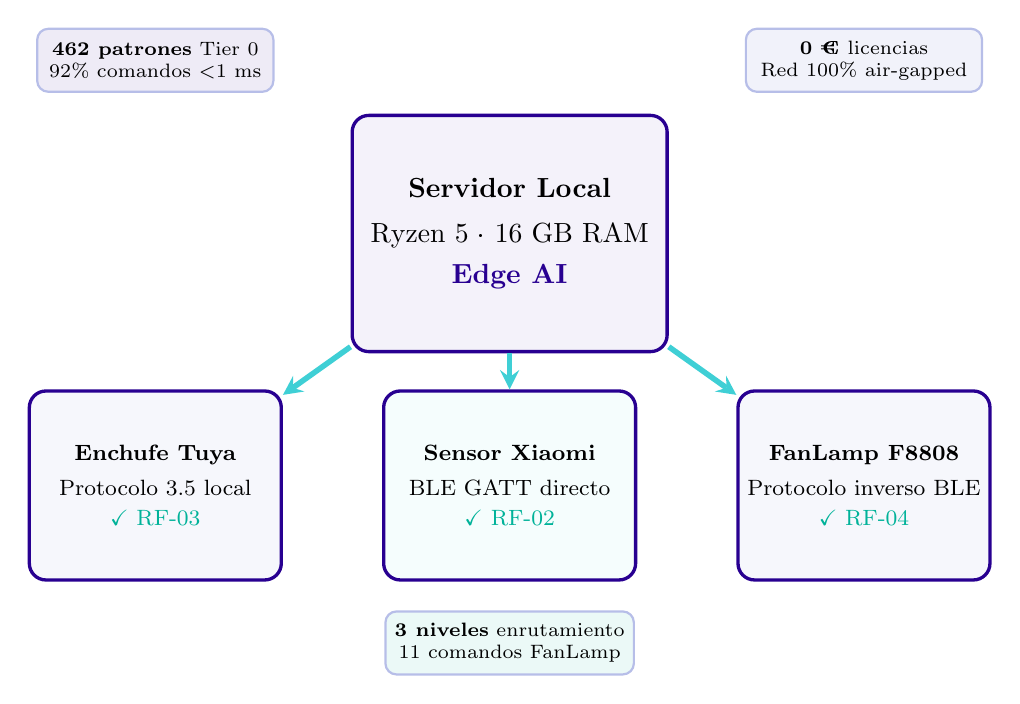
\begin{tikzpicture}[
    box/.style={draw=primary, fill=white, rounded corners=6pt,
                minimum width=3.2cm, minimum height=2.4cm, align=center,
                font=\footnotesize, line width=1.2pt},
    server/.style={box, minimum width=4cm, minimum height=3cm,
                   fill=primary!5, font=\normalsize},
    stat/.style={fill=secondary!8, draw=secondary!40, rounded corners=4pt,
                 minimum width=3cm, minimum height=0.8cm, align=center,
                 font=\scriptsize, line width=0.8pt},
    conn/.style={draw=accent, line width=2pt, ->, >=stealth},
]

% Servidor central
\node[server] (server) at (0,0) {
    \textbf{Servidor Local}\\[0.15cm]
    Ryzen 5 · 16 GB RAM\\[0.1cm]
    \textcolor{primary}{\textbf{Edge AI}}
};

% Dispositivos
\node[box, fill=secondary!5] (tuya) at (-4.5, -3.2) {
    \textbf{Enchufe Tuya}\\[0.1cm]
    {\footnotesize Protocolo 3.5 local}\\[0.05cm]
    {\footnotesize\color{exgreen}\checkmark\ RF-03}
};

\node[box, fill=accent!5] (xiaomi) at (0, -3.2) {
    \textbf{Sensor Xiaomi}\\[0.1cm]
    {\footnotesize BLE GATT directo}\\[0.05cm]
    {\footnotesize\color{exgreen}\checkmark\ RF-02}
};

\node[box, fill=secondary!5] (fanlamp) at (4.5, -3.2) {
    \textbf{FanLamp F8808}\\[0.1cm]
    {\footnotesize Protocolo inverso BLE}\\[0.05cm]
    {\footnotesize\color{exgreen}\checkmark\ RF-04}
};

% Conexiones
\draw[conn] (server) -- (tuya);
\draw[conn] (server) -- (xiaomi);
\draw[conn] (server) -- (fanlamp);

% Cifras clave en cajas flotantes
\node[stat, fill=primary!8] at (-4.5, 2.2) {
    \textbf{462 patrones} Tier~0\\
    92\% comandos $<$1 ms
};

\node[stat] at (4.5, 2.2) {
    \textbf{0 €} licencias\\
    Red 100\% air-gapped
};

\node[stat, fill=exgreen!8] at (0, -5.2) {
    \textbf{3 niveles} enrutamiento\\
    11 comandos FanLamp
};

\end{tikzpicture}
\end{document}
